\documentclass[12pt,a4paper,titlepage,listof=totoc,bibliography=totoc,chapteratlists=0pt]{scrreprt}

\begin{filecontents*}{\jobname.xmpdata}
	\Keywords{VR, IOT, TODO}
	\Title{Unser tolles Thema -- wir sind suppa}
	\Author{Stefan Schwammal, Susi Schwammal}
\end{filecontents*}
\setcounter{secnumdepth}{5}
\setcounter{tocdepth}{5}
%\renewcommand*\thesubsubsection{\arabic{subsubsection})}

\usepackage[utf8]{inputenc}
\usepackage[T1]{fontenc}
\usepackage{amsmath}
\usepackage{amsfonts}
\usepackage{amssymb}
\usepackage[table]{xcolor}
\usepackage{graphicx}
\usepackage[left=3.50cm, right=2.00cm, top=2.00cm, bottom=2.00cm,foot=1cm]{geometry}
\usepackage[splitrule,hang,flushmargin,multiple,bottom]{footmisc}
\usepackage{lmodern, textcomp}
\usepackage{lmodern}
\usepackage{pdfpages}
\usepackage[ngerman]{babel}
\usepackage{multicol}
\usepackage{subfig}
\usepackage{float}
\usepackage{array,tabularx,booktabs}
\usepackage{ragged2e}
\usepackage{lipsum}
\usepackage{wrapfig}


\newcolumntype{M}[1]{>{\centering\arraybackslash}m{#1}}

\usepackage{enumitem}
\newlist{compactitem}{itemize}{3}
\setlist[compactitem,1]{label=\textbullet, nosep,leftmargin=1.5em,labelwidth=*,align=left}
\setlist[compactitem,2]{label=--, nosep,leftmargin=1.5em,labelwidth=*,align=left}
\setlist[compactitem,3]{label=\textopenbullet, nosep,leftmargin=1.5em,labelwidth=*,align=left}
\newlist{compactenum}{enumerate}{3}
\setlist[compactenum,1]{label=\arabic*., nosep,leftmargin=1.5em,labelwidth=*,align=left}
\setlist[compactenum,2]{label=\alph*., nosep,leftmargin=1.5em,labelwidth=*,align=left}
\setlist[compactenum,3]{label=\roman*., nosep,leftmargin=1.5em,labelwidth=*,align=left}
\newlist{compactdesc}{description}{3}
\setlist[compactdesc]{leftmargin=1.5em,labelwidth=*,align=left}

\usepackage{microtype}

\usepackage[parfill]{parskip}

\definecolor{bluekeywords}{rgb}{0.13,0.13,1}
\definecolor{greencomments}{rgb}{0,0.5,0}
\definecolor{redstrings}{rgb}{0.9,0,0}
\definecolor{lightgray}{gray}{0.9}
\definecolor{lightblue}{rgb}{0.93,0.95,1.0}

\usepackage{listings}

\makeatletter
\lstdefinestyle{lststyle}{
	basicstyle=%
	\ttfamily
	\lst@ifdisplaystyle\scriptsize\fi
}
\makeatother

\renewcommand{\lstlistlistingname}{List of Listings}
% TODO: define other languages as needed
\lstset{language=Python,
numbers=left,               
numberstyle=\tiny,          
showspaces=false,
showtabs=false,
breaklines=true,
lineskip=-1pt,
tabsize=2,
showstringspaces=false,
breakatwhitespace=true,
escapeinside={(*@}{@*)},
commentstyle=\color{greencomments},
keywordstyle=\color{bluekeywords}\bfseries,
stringstyle=\color{redstrings},
style=lststyle,
xleftmargin=17pt,
         framexleftmargin=17pt,
         framexrightmargin=5pt,
         framexbottommargin=4pt
}
\lstset{
morekeywords={base,var,in,out,dynamic,from,where,select,orderby,function,\$,group,by,into,yield,async,await,@,None,self,as,elif,with}
}
\lstdefinelanguage{TypeScript}{
	keywords={typeof, new, true, false, catch, function, return, null, switch, var, if, in, while, do, else, case, break, void, number, string, boolean, module, \$, export, for, this},
	keywordstyle=\color{blue}\bfseries,
	ndkeywords={class, export, boolean, throw, implements, import, this},
	ndkeywordstyle=\color{darkgray}\bfseries,
	identifierstyle=\color{black},
	sensitive=false,
	comment=[l]{//},
	morecomment=[s]{/*}{*/},
	commentstyle=\color{purple}\ttfamily,
	stringstyle=\color{red}\ttfamily,
	morestring=[b]',
	morestring=[b]"
}
\usepackage{caption}
\DeclareCaptionFont{white}{\color{white}}
\DeclareCaptionFormat{listing}{\colorbox[cmyk]{0.43, 0.35, 0.35,0.01}{\parbox{\textwidth}{\hspace{10pt}#1#2#3}}}
\captionsetup[lstlisting]{format=listing,labelfont=white,textfont=white} 
\captionsetup[table]{justification=centering, singlelinecheck=false}

\usepackage{setspace}
\newcommand{\MSonehalfspacing}{%
	\setstretch{1.44}%  default
	\ifcase \@ptsize \relax % 10pt
	\setstretch {1.448}%
	\or % 11pt
	\setstretch {1.399}%
	\or % 12pt
	\setstretch {1.433}%
	\fi
}

\newcommand{\setauthor}[1]{\ohead[]{#1}}

\usepackage[automark]{scrlayer-scrpage}
\pagestyle{scrheadings}
\automark{chapter}
\renewcommand\sectionmark[1]{\markright{\MakeMarkcase {\thesection\hskip .5em\relax#1}}}
\rohead{\ifnum\expandafter\pdfstrcmp\botmark=0 \rightmark\else\leftmark{} --- \rightmark\fi}
\ihead[]{\headmark}
\chead[]{}
\ohead{}
\cfoot[]{}
\ofoot[\pagemark]{\pagemark}
\setheadsepline{.1pt}

\usepackage[hyphens]{url}

\usepackage[a-1b]{pdfx}

\usepackage{hyperref}
\hypersetup{pdfa}

\usepackage[nonumberlist,toc,nopostdot]{glossaries}

\usepackage{chngcntr}
\counterwithout{footnote}{chapter}
\counterwithout{figure}{chapter}
\counterwithout{table}{chapter}
\AtBeginDocument{
	\counterwithout{lstlisting}{chapter}
	\urlstyle{sf}
}
\newcounter{RPages}

\makeatletter
\def\bstctlcite{\@ifnextchar[{\@bstctlcite}{\@bstctlcite[@auxout]}}
\def\@bstctlcite[#1]#2{\@bsphack
	\@for\@citeb:=#2\do{%
		\edef\@citeb{\expandafter\@firstofone\@citeb}%
		\if@filesw\immediate\write\csname #1\endcsname{\string\citation{\@citeb}}\fi}%
	\@esphack}
\makeatother

\clubpenalty=10000
\widowpenalty=10000
\displaywidowpenalty=10000
\interfootnotelinepenalty=10000

\title{Unser tolles Thema -- wir sind suppa}
\author{Stefan Schwammal, Susi Schwammal}

\makeindex
\makeglossaries
\begin{document}
\bstctlcite{IEEEexample:BSTcontrol}
\newcommand{\reminder}[1]
{ \textcolor{red}{<[{\bf\marginpar{\mbox{$<==$}} #1 }]>} }
\newcommand{\icode}[1]{\lstinline$#1$}
%\urlstyle{same}
%\setstretch{1.5}
\setstretch {1.433}
\renewcommand{\arraystretch}{1.2}


\includepdf{./titlepage/coversheet}
\pagenumbering{Roman}
\newpage
\thispagestyle{empty}
\vspace{3cm}
~ \\ \\

Ich erkläre an Eides statt, dass ich die vorliegende Diplomarbeit selbstständig und ohne fremde Hilfe verfasst, andere als die angegebenen Quellen und Hilfsmittel nicht benutzt bzw. die wörtlich oder sinngemäß entnommenen Stellen als solche kenntlich gemacht habe.

Die Arbeit wurde bisher in gleicher oder ähnlicher Weise keiner anderen Prüfungsbehörde vorgelegt und auch noch nicht veröffentlicht.

Die vorliegende Diplomarbeit ist mit dem elektronisch übermittelten Textdokument identisch.
\vspace{3cm}
% Hier kommt die Unterschrift drüber
\begin{tabbing}
Leonding, April 2022 \hspace{5cm} S. Schwammal \& S. Schwammal
\end{tabbing}
\vspace{10cm}
Zur Verbesserung der Lesbarkeit wurde in diesem Dokument auf eine geschlechtsneutrale Ausdrucksweise verzichtet.
Alle verwendeten Formulierungen richten sich jedoch an beide Geschlechter.
\newpage
\setcounter{page}{1}
\begin{spacing}{1}
    \chapter*{Abstract}
\end{spacing}
The automation and centralization of the input of information helps to organize various tasks and activities quickly,
efficiently and in a resource-saving manner. 
HTL Leonding is confronted with the organization of module registrations and school attendance and AMS confirmations every year. 


The goal of this thesis is to implement a web application that digitizes the organizational tasks of HTL Leonding.
The choice of the framework and the database system play an important role. Different systems were tested for performance,
functionality and popularity with developers. 
The present software was developed with the Angular front-end web application framework and an Oracle SQL database in the back-end. 
The software not only accelerated data processing, but also made the dataset clearer and prepared it for future statistical analysis.

\newpage
\begin{spacing}{1}
    \chapter*{Zusammenfassung}
\end{spacing}
\begin{wrapfigure}{r}{0.3\textwidth}
\end{wrapfigure}
Die Automatisation und Zentralisation der Eingabe von Informationen trägt dazu bei, die Organisation verschiedener Aufgaben und Tätigkeiten schnell,
effizient und ressourcenschonend zu erledigen. 

Die HTL Leonding ist jedes Jahr mit der Organisation der Modulanmeldungen und der Schulbesuchs- und AMS-Bestätigungen konfrontiert. 

Das Ziel der vorliegenden Arbeit ist es, eine Web-Anwendung zu implementieren, die die organisatorischen Aufgaben der HTL Leonding digitalisiert.
Dabei spielen die Wahl des Frameworks und des Datenbanksystems eine wichtige Rolle. Verschiedene Systeme wurden auf Performance, Funktionalität und Beliebtheit bei Entwicklern untersucht. 

Die vorliegende Software wurde mit dem Angular Front-End Webapplikations-Framework und einer Oracle SQL-Datenbank im Back-End entwickelt. 

Durch die Software wurde nicht nur die Datenverarbeitung beschleunigt, sondern auch der Datenbestand übersichtlicher gestaltet und für zukünftige statistische Auswertungen aufbereitet.




\pagestyle{plain}

\renewcommand{\lstlistlistingname}{Quellcodeverzeichnis}

\tableofcontents
\newpage
\setcounter{RPages}{\value{page}}
\setcounter{page}{0}
\pagenumbering{arabic}
\pagestyle{scrheadings}

\begin{spacing}{1}
	\chapter{Einleitung}\label{chapter:einleitung}
\end{spacing}
\section{Ist Situation}
\setauthor{Emir Bajramovic}
\lipsum[5-12]

\section{Abendschule}
\setauthor{Emir Bajramovic}
\lipsum[12-18]

%------------------------------------------------------------

\begin{spacing}{1}
	\chapter{Problemstellung}\label{chapter:problemstellung}
\end{spacing}
\section{Modulesystem}
\setauthor{Emir Bajramovic}
\lipsum[5-12]


\section{Bestätigunssystem}
\setauthor{Emir Bajramovic}
\lipsum[5-12]
%------------------------------------------------------------

\begin{spacing}{1}
	\chapter{Umfeldanalyse}
\end{spacing}
\lipsum[4] Citing properly.

Was ist eine \gls{guid}?
Eine \gls{guid} kollidiert nicht gerne.

Kabellose Technologien sind in abgelegenen Gebieten wichtig.

%------------------------------------------------------------

\begin{spacing}{1}
	\chapter{Technologische Hintergrund}\label{chapter:tech}
\end{spacing}
\section{Auswahl des Datenbank-Systems}
    \setauthor{Sandor Debnar}
    
\begin{spacing}{1}  
\end{spacing}
Die Auswahl der Entwicklungsumfeld spielt bei jedem Softwareprojekt eine sehr
wichtige Rolle. Großer Anteil der Frameworks bieten unterschiedliche Vorteile,
Funktionen. 
Das Entwicklungsteam ist für die Prüfung und Auswahl der Software verantwortlich,
die den Projektanforderungen entspricht. In den folgenden Kapiteln werden
die Hintergründe und Kriterien für die Auswahl der Front- und Backend Programmen
beschrieben. 
    \subsection{Datenbank}
        Die hier vorgestellte Software wird eine große Menge von Schüler- und Moduldaten verarbeiten, die in strukturierten und effizienten  
Tabellen in einer relationalen Datenbank gespeichert werden. Dieses RDBMS (Relationale Datenbank Management System) wird eine Schnittstelle 
zwischen Nutzern und Anwendungen bilden, die für Verwaltungs-, Zugangs- und Performancefunktionen anbietet. In den folgenden Unterabschnitten 
werden die gängigsten Datenbanken vorgestellt und anhand ihrer Hauptmerkmale die Datenbanken ermittelt, die den Anforderungen des Projekts am 
besten entsprechen. Die Unterschiede zwischen den drei führenden Datenbanken sind nicht so ausgeprägt, so dass der Vergleich zwischen
der beliebtesten und der mäßig bekannten Software erfolgt. Die Auswahl basierte auf den Kriterien von DB-Engines.com für das Ranking 
der Datenbanken, d. h. auf der Anzahl der Erwähnungen auf Websites, dem durchschnittlichen Interesse an dem System, der Häufigkeit 
von Fachdiskussionen über das System, Stellenanzeigen, die das System erfordern, und der Relevanz in sozialen Medien. 
Siehe Abbildung \ref{db_engines_ranking}
\begin{figure}[h]
    \begin{center}
        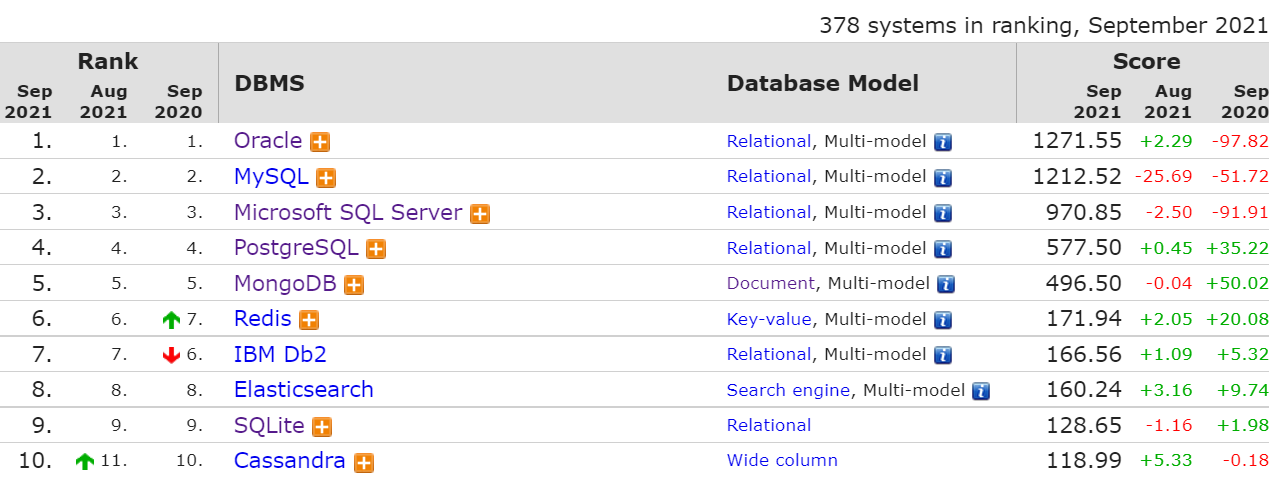
\includegraphics[scale=0.5]{./pics/db_engines_ranking.png}
        \caption{Db-Engines Ranking}
        \label{db_engines_ranking}
    \end{center}
\end{figure}
\newpage
    \subsection{SQLite}
        Diese Datenbank wurde von Dwayne Richard Hipp in den frühen 2000er Jahren entwickelt und bietet ein relationales,
leichtgewichtige Datenbankmanagementsystem ohne sekundäre Datenbankmodelle. Einer der Hauptvorteile ist die Tatsache,
dass es sich um eine Open-Source-Datenbank für mehrere Plattformen (Windows, Mac, Linux, Unix usw.) handelt, die dank der einfachen Datenspeicherung,
der dynamischen Datentypen und einer breiten Palette von Programmiersprachen (VS Basic, C-sharp, PHP, Python usw.) eine schnelle und einfache Lösung für die Speicherung von Daten bietet.


\begin{large} \emph{\textbf{Hauptmerkmalen}} \end{large}
\begin{itemize}
    \item \underline{\texttt{Portabilität}}:
        SQLite speichert seine Datenbank in einer normalen Festplattendatei 
        innerhalb des Verzeichnisses,
        was es zu einem der portabelsten RDBMS macht. 
    \item \underline{\texttt{Unterstützte Datensätze}}:
        die grundlegenden Datentypen sind 64-Bit-Integer, 64-Bit-IEEE-Gleitkommazahl,
        String, TEXT, BLOB, NULL. 
    \item \underline{\texttt{Eigenständig}}:
        nicht vom Betriebssystem oder externen Bibliotheken abhängig und kann aufgrund seines geringen
        Speicherplatzbedarfs (500KB) in einer Vielzahl von Umgebungen eingesetzt werden, einschließlich 
        mobiler Geräte (Android, iPhone) und Spielkonsolen.
    \item \underline{\texttt{Geschwindigkeit}}:
        SQLite schneidet bei den folgenden Abfragen gut ab (insbesondere, wenn sie in einer Transaktion sind),
        dank seiner kompakten, einfachen Architektur und Gestaltung.
    \item \underline{\texttt{Serverlos}}:
        keine Client-Server-Architektur ist erforderlich, so dass es innerhalb der Anwendung arbeiten kann. 
    \item \underline{\texttt{Zero Konfiguration}}:
        keine Installations- oder Serveranforderungen von dem Benutzer erforderlich und es ohne Datenbankkonfiguration
        verwendet werden kann. 
    \item \underline{\texttt{Transaktional}}:
        Transaktionen folgen der A-C-I-D-Struktur für Zuverlässigkeit, was bedeutet, dass die meisten Abfrageeigenschaften
        den Grundsätzen der Atomarität, Konsistenz, Isolierung und Dauerhaftigkeit entsprechen.  
    \item \underline{\texttt{Online Backup-API}}:
        Die Online-Backup-API, der einzige Datenwiederherstellungsmechanismus, der es ermöglicht, Daten von einer Datenbank
        in eine andere zu kopieren, sogar inkrementell, indem der Inhalt der Zieldatenbank unter Verwendung von Shared-Locks überschrieben wird.
\end{itemize} 
\begin{large} \emph{\textbf{Fazit}} \end{large}
    SQLite ist eine leicht einzurichtende, schnelle und benutzerfreundliche Datenbank, deren Schwäche jedoch ihre Einfachheit ist.
    Mit zunehmender Komplexität der Aufgaben werden Unzulänglichkeiten wie die Verarmung der Datentypen, fehlende Sicherheitsmechanismen
    für Daten und Backups, nicht unterstützte Dateiformate (XML), fehlender Mehrfachzugriff und fehlende erweiterte Funktionen immer deutlicher.  
        \newpage
    \subsection{PostgreSQL}
        Die Datenbank wurde um 1986 an der Universität von Kalifornien in Berkeley entwickelt.
Die Software ist eine Open-Source Objekt-RDBMS. Das System gewährleistet die Datenintegrität 
unabhängig von der Datengröße und ist zudem in hohem Maße erweiterbar, z. B. mit benutzerdefinierten
Datensätzen, Funktionen, sekundäre Datenbankmodellen und sogar verschiedenen Programmiersprachen, 
ohne dass die Datenbank neu kompiliert werden muss. PostgreSQL ist eine komplexere Datenbank als
SQLite in Bezug auf Funktionen, unterstützte Datentypen und Zuverlässigkeit. \cite{PostgreSQL_About}

\begin{large} \emph{\textbf{Hauptmerkmalen}} \end{large}
\begin{itemize}
    \item \underline{\texttt{Portabilität}}:
        PostgreSQL ist nur portabel, wenn die Datenbank in eine Datei exportiert und dann
        auf einen Server kopiert wird. \cite{SQLite_vs_PostgreSQL}
    \item \underline{\texttt{Unterstützte Datensätze}}:
        Das Programm kann jeden Datentyp speichern, der in einer Datenbank vorkommen
        kann. \cite{SQLite_vs_PostgreSQL}
    \item \underline{\texttt{Datenbankmodell}}:
        die PostgreSQL-Datenbank benötigt mehr Speicherplatz (200 MB), da sie ein 
        Client-Server-Modell darstellt und einen Datenbankserver zur Installation und 
        Ausführung benötigt.\cite{SQLite_vs_PostgreSQL}
    \item \underline{\texttt{Sicherheit}}:
        PostgreSQL bietet mehrere Datensicherheitsmechanismen, z.B. GSSAPI, SSPI, LDAP, 
        um sensible Daten zu schützen.\cite{PostgreSQL_Authentication}
    \item \underline{\texttt{Standardisiert}}:
         PostgreSQL unterstützt 160 der 190 grundlegenden SQL-Features.\cite{PostgreSQL_standardisierung}
    \item \underline{\texttt{Backup}}:
        PostgreSQL bietet drei verschiedene Backup-Strategien: SQL Dump, File System 
        Level Backup und kontinuierliche Archivierung.\cite{PostgreSQL_Backup}
\end{itemize} 
\begin{large} \emph{\textbf{Fazit}} \end{large}
PostgreSQL verfügt über zusätzliche Funktionen, die für Integrität und Sicherheit sorgen,
sowie über die Portabilität, um komplexe Datenbanken problemlos zu betreiben. Der Preis
dafür ist ein erhöhter anfänglicher Ressourcenbedarf, sowohl in Bezug auf den 
Arbeitsspeicher als auch auf den Speicherplatz, und eine umständlichere Implementierung. 
    \subsection{MySQL}
        MYSQL wurde erstmals 1944 von einem schwedischen Unternehmen entwickelt und die erste Version
wurde 1945 veröffentlicht. Das Unternehmen wurde in 2008 von Sun Microsystem und in 2010 von seinem
heutigen Eigentümer Oracle übernommen.\cite{MySQL_Wiki}

MySQL ist ein reines RDBMS, das in seinen kostenpflichtigen Paketen neben den Basisdiensten 
zusätzliche Funktionen und die neuesten technologischen Entwicklungen bietet. 

\begin{large} \emph{\textbf{Hauptmerkmalen}} \end{large}
\begin{itemize}
    \item \underline{\texttt{Portabilität}}:
        Die in C und C++ geschriebene Software funktioniert nicht nur in Umgebungen,
        die mit verschiedenen Compilern getestet wurden, sondern auch auf einer Vielzahl 
        von Betriebssystemen und kann problemlos mit der Software CMake portiert werden.\cite{MySQL_Features}
    \item \underline{\texttt{MVCC}}:
        Die Datenbankfunktionen folgen der MVCC-Architektur (Multi-Version Concurrency Control),
        so dass Datenbankzugriffe mit gleicher Priorität effizient durchgeführt werden können, 
        ohne die Datenbank zu blockieren oder ihre Konsistenz zu gefährden.\cite{MVCC_Wiki}
    \item \underline{\texttt{Unterstützte Datensätze}}:
        Die Software unterstützt nicht nur die meisten Datentypen, sondern bietet auch spezielle 
        Funktionen wie das Referenzieren von Tabellen in anderen Datenbanken.\cite{MySQL_Features}
    \item \underline{\texttt{Sicherheit}}:
        MySQL bietet auch Sicherheitsmechanismen zum Schutz der Daten. 
        (SHA-2, PAM, LDAP, Kerberos usw.) \cite{MySQL_Authentication}
    \item \underline{\texttt{Storage Engines}}:
        Sind Komponenten, die vom System für verschiedene Operationen verwendet werden kann.
        Die unterstützten Engines sind InnoDB, MyISAM, Memory, CSV, Archive, Blackhole, NDB,
        Merge, Federated, Example. \cite{MySQL_Storage_Engines}
    \item \underline{\texttt{Servereinstellungen}}:
        Die Datenbank bietet die Möglichkeit, Festplatten I/O, Speichernutzung, Dateilayout und 
        Systemfaktoren wie External Locks zu optimieren.\cite{MySQL_Server_Optimalization}
    \newpage
    \item \underline{\texttt{Backup und Recovery}}:
        MySQL bietet eine Reihe von Varianten für Backup-Strategien, wie z. B. physische und logische
        Backups, Online- und Offline-Backups, lokale und Remote-Backups, Snapshot-Backups sowie
        vollständige und inkrementelle Backups.\cite{MySQL_Backup}
\end{itemize} 
\begin{large} \emph{\textbf{Fazit}} \end{large}
MySQL ist ein einfaches RDBMS mit den meisten Funktionen, die für moderne Datenbanken erforderlich 
sind, sowohl in Bezug auf Sicherheit, Integrität und Flexibilität. Häufige Aktualisierungen und neue
Funktionen sind nicht nur für kostenpflichtige Pakete verfügbar, so dass es sich wirklich um eine
kostenlose Open-Source-Datenbank handelt. 
        \newpage
    \subsection{Fazit}
    \lipsum[5-8]
\section{Auswahl des Frontend Frameworks}
    \lipsum[5-12]
    \subsection{.Net}
        \lipsum[5-12]
    \subsection{.Net Core MVC}
        \lipsum[5-12]
    \subsection{ASP.Net - Angular}
        \lipsum[5-12]
\section{Server}
    \lipsum[5-12]
    \subsection{Webhosting Lösungen}
        \lipsum[5-12]
    \subsection{Microsoft Azure}
        \lipsum[5-12]

%------------------------------------------------------------

\begin{spacing}{1}
	\chapter{Technische Umsetzung}\label{chapter:implementation}
\end{spacing}
Siehe tolle Daten in Tab. \ref{tab:impl:data}.

\begin{table}
    \centering
    \begin{tabular}{|lcc|}
    \hline
              & \textbf{Regular Customers} & \textbf{Random Customers} \\ \hline
    Age       & 20-40                      & \textgreater{}60          \\ \hline
    Education & university                 & high school               \\ \hline
    \end{tabular}
    \caption{Ein paar tabellarische Daten}
    \label{tab:impl:data}
\end{table}

\begin{figure}
    \centering
    
\includegraphics[scale=0.5]{pics/knuthi.jpg}
    \caption{Don Knuth -- CS Allfather}
    \label{fig:impl:knuth}
\end{figure}

Siehe und staune in Abb. \ref{fig:impl:knuth}.
\lipsum[6-9]
Dann betrachte den Code in Listing \ref{lst:impl:foo}.

\begin{lstlisting}[language=Python,caption=Some code,label=lst:impl:foo]
# Program to find the sum of all numbers stored in a list (the not-Pythonic-way)

# List of numbers
numbers = [6, 5, 3, 8, 4, 2, 5, 4, 11]

# variable to store the sum
sum = 0

# iterate over the list
for val in numbers:
    sum = sum+val

print("The sum is", sum)
\end{lstlisting}
%------------------------------------------------------------

\begin{spacing}{1}
	\chapter{Tools der Projektentwicklung}\label{chapter:tools}
\end{spacing}

\subsection{Agile Methoden}
\setauthor{Thomas Straßhofer}
    \lipsum[5-7]
\subsection{GitHub}
    \lipsum[5-7]

%------------------------------------------------------------

\newpage
\pagenumbering{Roman}
\setcounter{page}{\value{RPages}}
\newacronym{guid}{GUID}{Globally Unique Identifier}
\newacronym{jit}{JIT}{Just In Time Compiler}
\newacronym{nfc}{NFC}{Near Field Communication}
\newacronym{rfid}{RFID}{Radio Frequency Identification}

% Usage:
% \gls{label} lowercase in text
% \Gls{label} Uppercase in text
% \newacronym{label}{abbrev}{full}
% \newglossaryentry{label}{settings}



%\setlength{\glsdescwidth}{0.8\linewidth}
\glsnogroupskiptrue
\printglossary[title=Glossar,toctitle=Glossar] %,style=long]
\spacing{1}{
	%\bibliographystyle{IEEEtran}
	\bibliographystyle{ieeetrande}
	\bibliography{bib}
}
\listoffigures
\listoftables
\lstlistoflistings
\appendix
\addchap{Anhang}
\input{./sections/appendix}
\end{document}

